\documentclass[12pt]{article}
\usepackage[utf8]{inputenc}

\title{COMP 138 RL: Homework 1}
\author{Erli Cai}

\usepackage{subcaption}
\usepackage{graphicx}
\graphicspath{ {./images/} }
\usepackage[fleqn]{amsmath}
\begin{document}

\maketitle

\section{Motivation}
In textbook, we have mainly focused our study on stationary bandit problems and on investigating performance of different algorithms on stationary problem. However, we don't no how these algorithms performs on a nonstationary problem. Therefore, in this programming task, I want to investigate the difficulties that sample-average methods have for nonstationary problem.


\section{Background}
\subsection{Non-stationary K-Armed Bandit}
In Machine Learning, a k-armed bandit problem  is a problem in which a fixed limited set of resources must be allocated between competing (alternative) choices in a way that maximizes their expected reward, when each choice's properties are only partially known at the time of allocation, and may become better understood as time passes or by allocating resources to the choice.$^{[1]}$ On top of that, we will be interested in non-stationary k-armed bandit, meaning that the reward function for each action is not  a stationary probability distribution but a probability distribution with varying distribution.


\subsection{Action-Value Methods}
In our k-armed bandit problem, each of the k actions has an expected or mean reward given that that action is selected; we call this the value of that action and denote it as $q_*(a)$ where $q_*(a) = E[R_t |A_t = a]$. In most cases, we don't know the action values with certainty and we want to estimate the value of action a at time step t as $Q_t(a)$. We would like $Q_t(a)$ to be close to $q_*(a)$. Among the several ways to estimate the value function, we are interested in action-value method using sample average and action-value method using constant step size.

\subsection{Sample average vs constant step size}
The difference between sample average method and constant step size method is that we estimate $q_*$ using different formula \\
Sample Average:$Q_{n+1} = \frac{R_1+R_2+...+R_{n}}{n} = Q_{n} + \frac{1}{n+1}[R_n-Q_n]$\\
Constant step size: $Q_{n+1} = Q_{n} +\alpha[R_n-Q_n]$ with $\alpha \in (0,1]$\\
We can easily see that these two methods put different weight on future rewards, with constant step size put more weight on future rewards. This is essentially what makes it more suitable for nonstationary bandit problem.


\section{Implementation}
We test the performance of each method on a ten arm bandits with each arm start with a normal distribution centered at 0 and has standard distribution 1. The mean value of each arm then takes random walk with mean zero and standard deviation 0.01 on each step. we record the reward of first 10,000 steps and repeat for 1000 times and take the average as performance.\\

It should be noted that, there is a lot of randomness involved in random walk. If we test the two methods on two bandit machine separately, the difference in performance could well come from this randomness. To eliminate the effect of this randomness on our comparison, in each trial, we simulate two agents deploying different strategy and only one bandit machine. Since each agents choice of action has not effect on bandit machine, we can be assured that agents won't affect the decition of each other.


\section{Result}
Figure 1 show the result of running 1000 simulation of ten armed bandit machine with the following parameter value:\\
\begin{itemize}
\item $\epsilon = 0.1$
\item $\alpha = 0.1$
\item standard deviation of each arm = 1
\item mean of each arm: random walk with mean zero and standard deviation 0.01 
\end{itemize}

Figure 1 shows the result of 4 trails of the performance against steps over first 10000 steps. These results are picked randomly among the 1000 simulations we do. We can see that the result varies dramatically, in some cases(subgraph c) sample average method performs better while in others constant step size method performs better.\\

This variation of result is due to the fact that the mean of each arm takes random walk over real number. In theory, the distance between mean of each arm and 0 should takes approximately normal distribution in a long run and this can be affirmed by Figure 2, where we draw the probability density function of bandits’ real mean value after 10000 steps . To eliminate the randomness introduced by random walk, we take average over 1000 trials as performance of each method. Although we will lost the information about individual trials, we can see that the difference in performance becomes more significant(as shown in Figure 3)
\\

In Figure 3, we can see that after 10000 steps, the average reward over 1000 trials for using sample average method is about 0.4 while average rewards for using constant step size is 0.85. we can conclude that constant step method perform significantly better than sample average method. 


\begin{figure}
\begin{subfigure}{.5\textwidth}
  \centering
  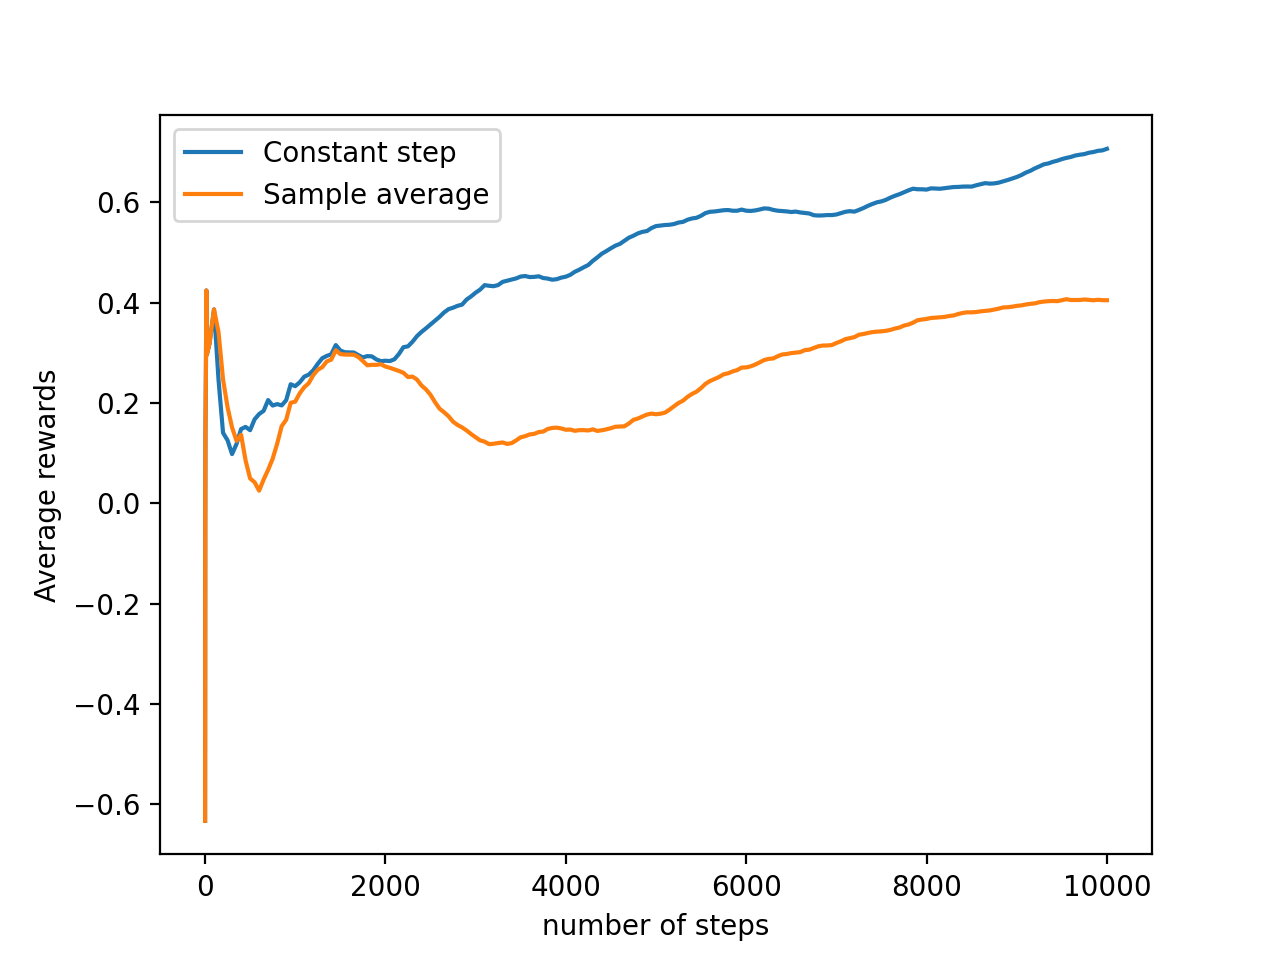
\includegraphics[width=1.1\linewidth]{Figure_2.png}
  \caption{}
\end{subfigure}%
\begin{subfigure}{.5\textwidth}
  \centering
  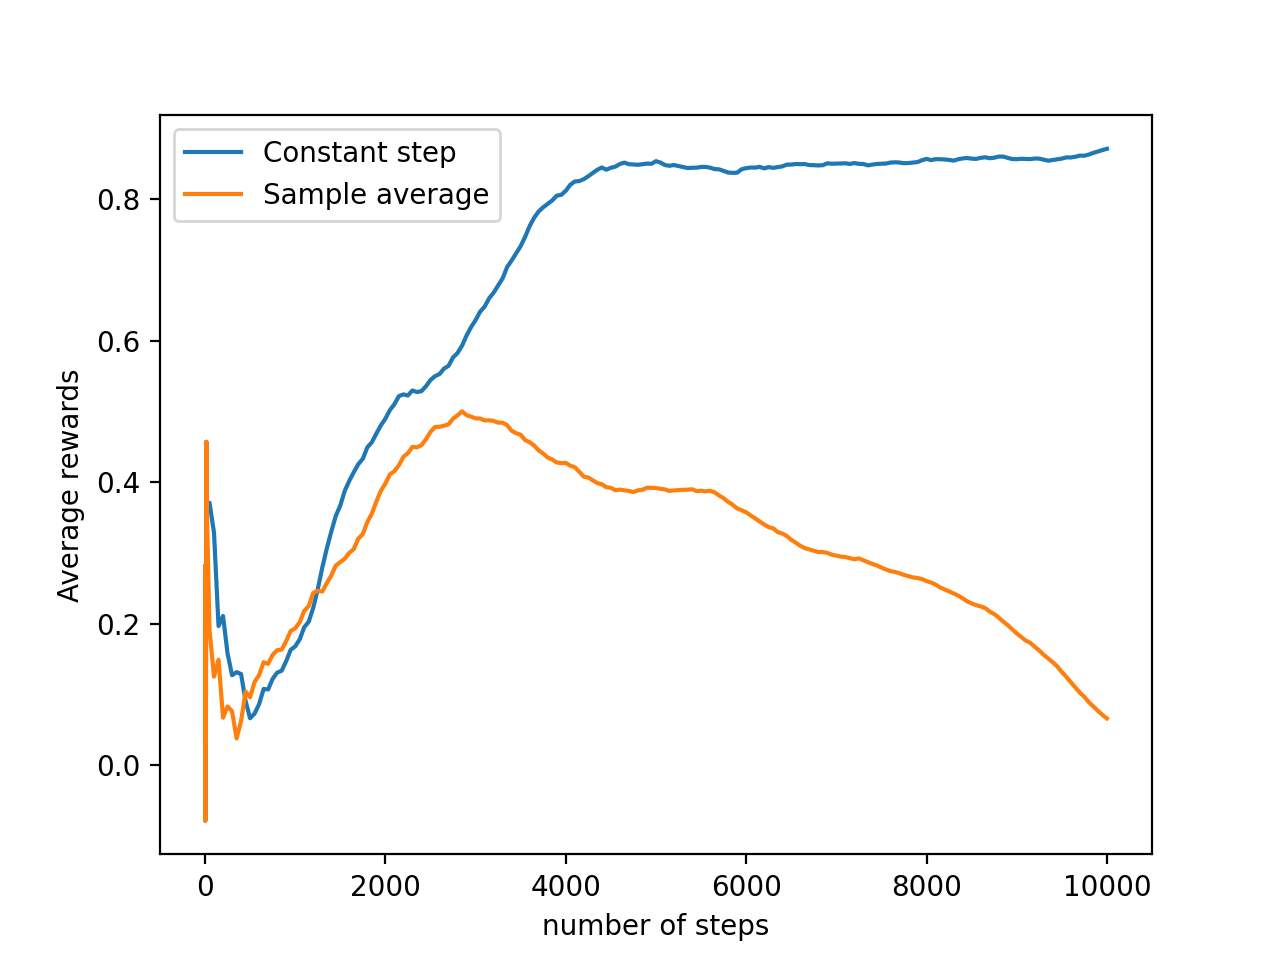
\includegraphics[width=1.1\linewidth]{Figure_3.png}
  \caption{}
\end{subfigure}
\begin{subfigure}{.5\textwidth}
  \centering
  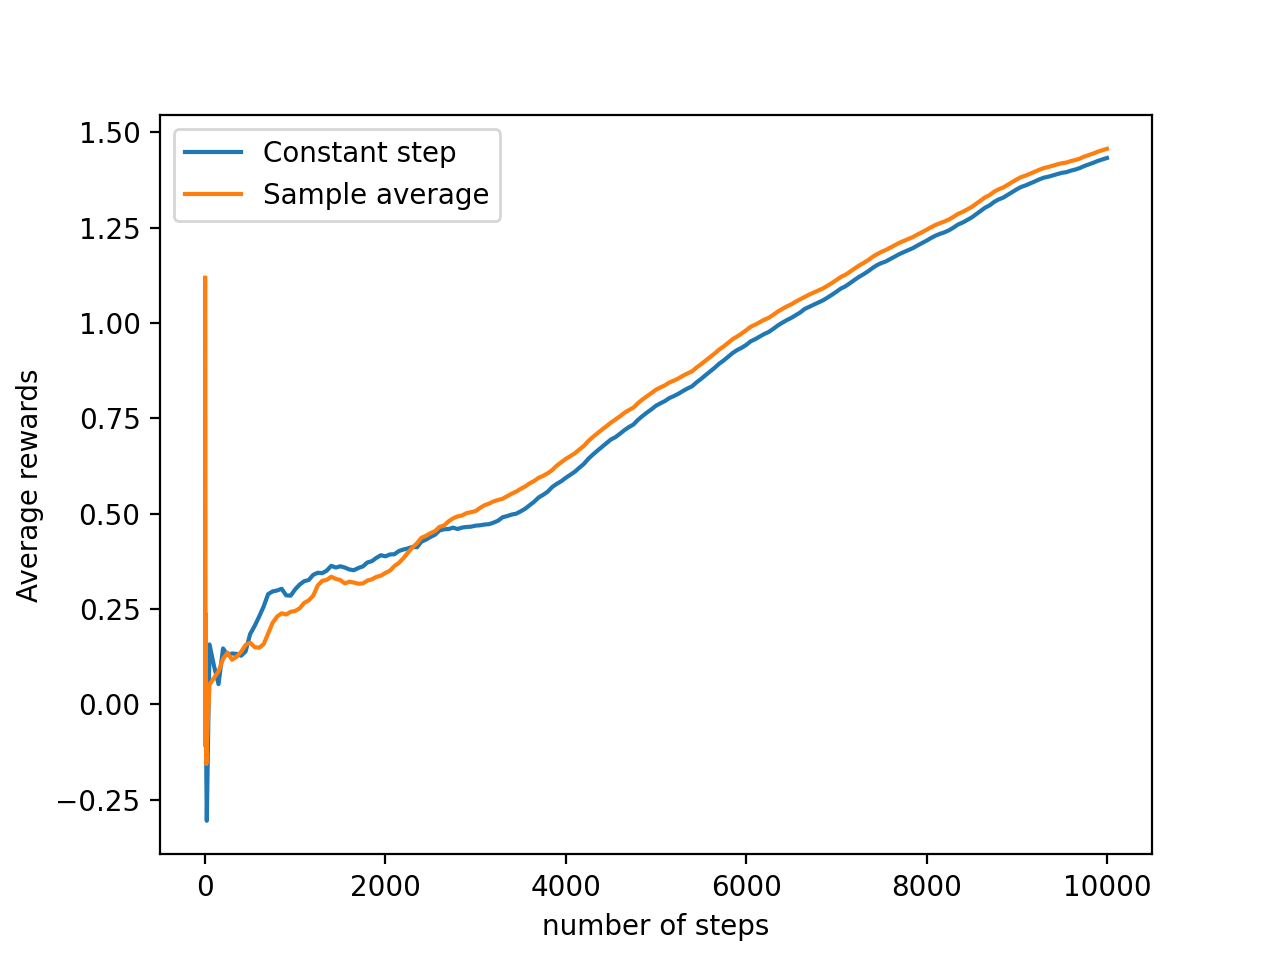
\includegraphics[width=1.1\linewidth]{Figure_4.png}
  \caption{}
\end{subfigure}%
\begin{subfigure}{.5\textwidth}
  \centering
  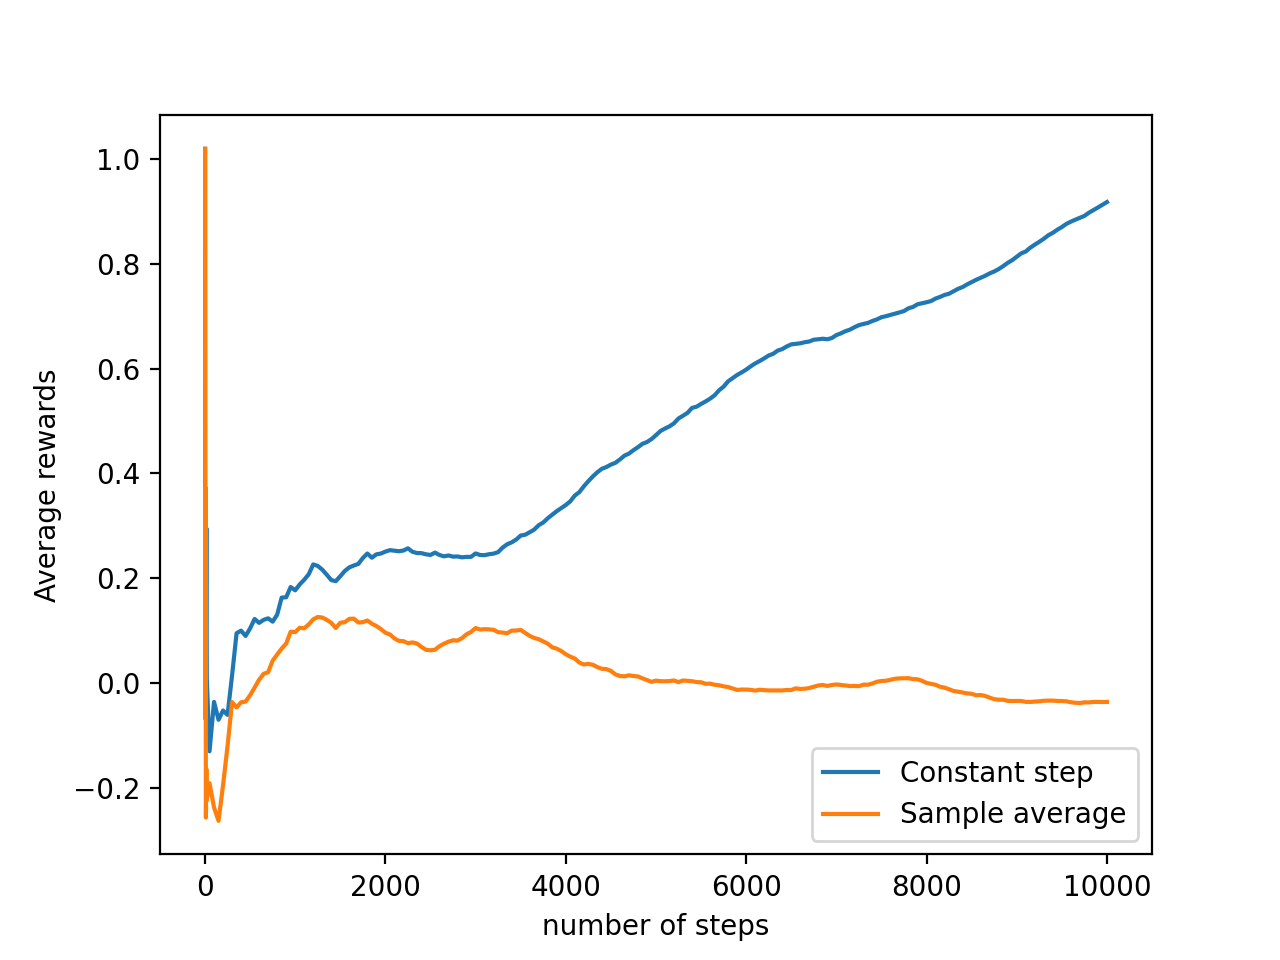
\includegraphics[width=1.1\linewidth]{Figure_5.png}
  \caption{}

\end{subfigure}
\caption{Performance over steps for constant step method(blue) and sample average method(orange) in first 10000 steps in 1 trial with parameters $\alpha = 0.1, \epsilon = 0.1$. These trials are picked randomly from our experiment data.}
\label{fig:fig}
\end{figure}

\begin{figure}
  \centering
     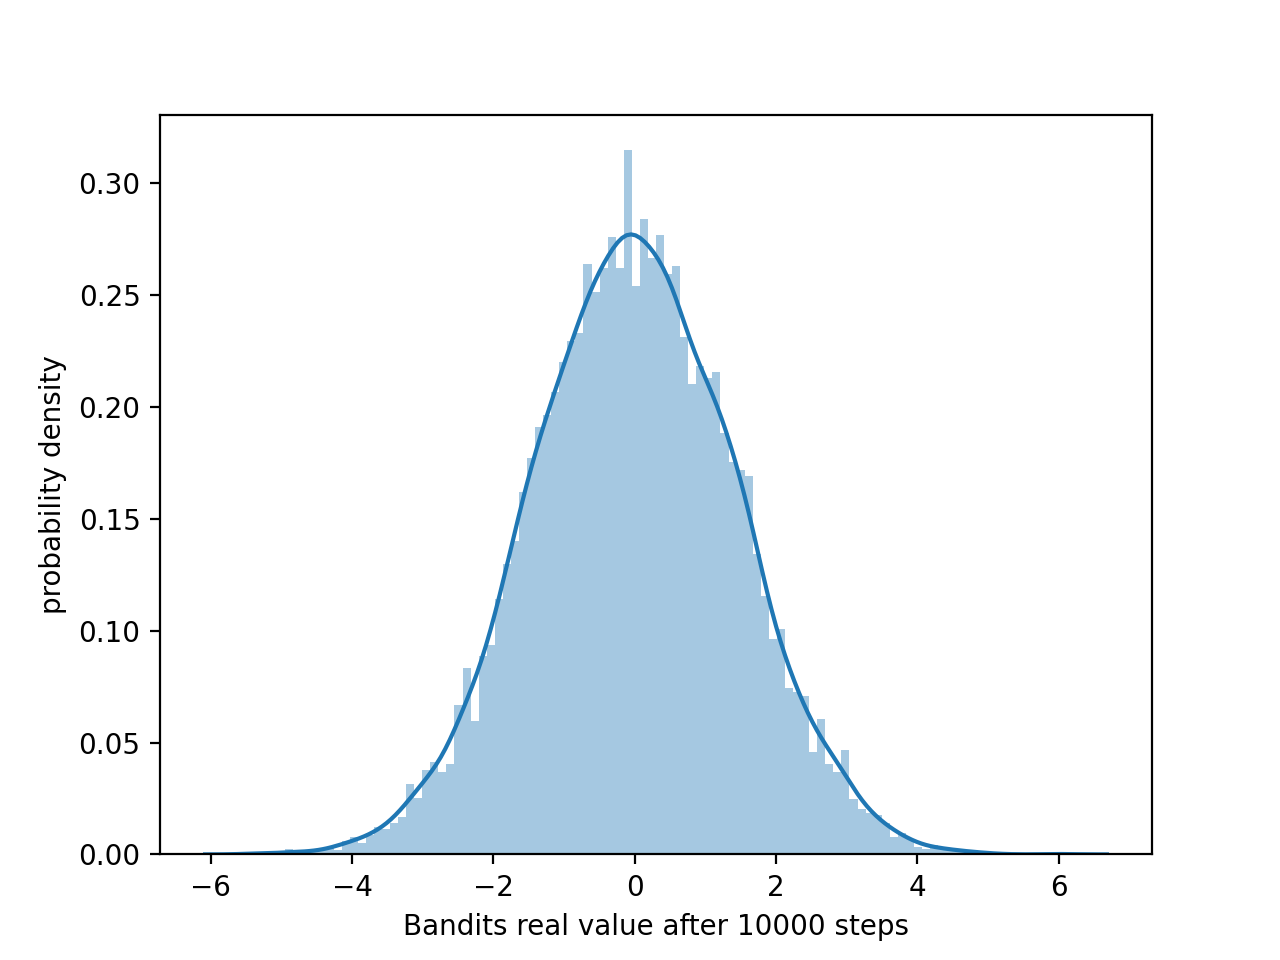
\includegraphics[width=\textwidth]{Figure_6.png}
  \caption{Probability density function of bandits' real mean value after 10000 steps}
\end{figure}


\begin{figure}
  \centering
     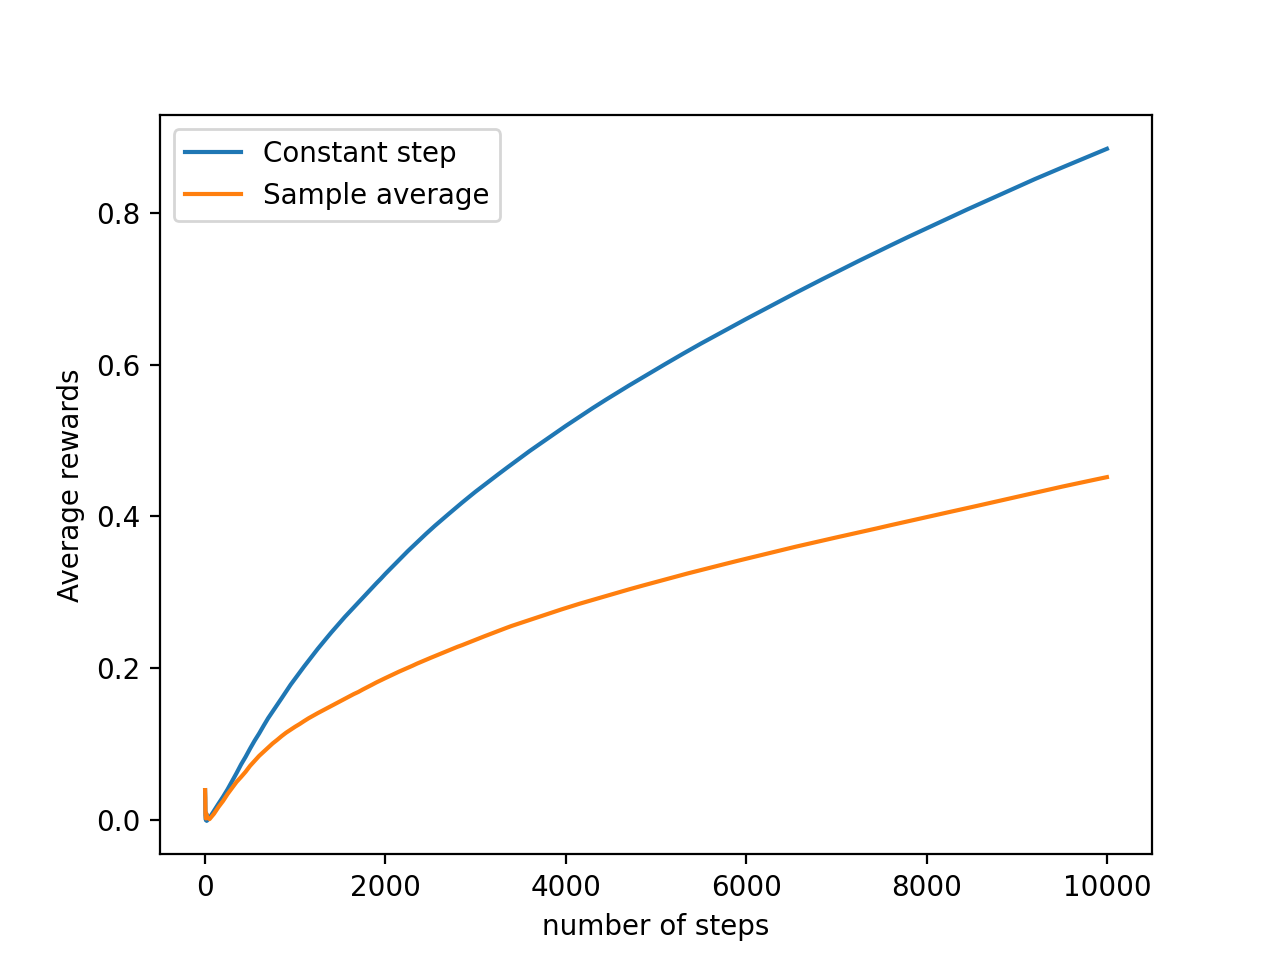
\includegraphics[width=\textwidth]{Figure_1.png}
  \caption{Performance over steps for constant step method(blue) and sample average method(orange) in first 10000 steps averaged over 1000 trials with parameters $\alpha = 0.1, \epsilon = 0.1$  }
\end{figure}



\pagebreak

\section{Discussion}
\subsection{Explanation of Experiment result}
We have seen that in a nonstationary bandit problem, sample average method perform worse than constant step size method. This is because sample average method put decrease weight on future reward. In this setting, if one bandit change from the optimal choice to suboptimal choice due to random walk of its mean value, it would take longer for sample average method to find out about this change. \\

\subsection{Further Experiment}
After seeing that sample-average method performs way worse than constant step size method on nonstationary bandit problem, I was wondering how other method we applied to stationary problem ( namely UCB method, optimistic initial value method and gradient bandit method) will behave in this setting. So I conduct the following experiment to investigate into these different methods.\\

We applied the same approach to Optimistic initial values method, UCB method, gradient bandit method, sample average method, constant step size method. The performance of each method in first 10000 steps is can be found in Figure 4. It should be noted that there is no guarantee that Optimistic initial value method, UCB method and gradient bandit method are at their best performance since I just choose one value for each parameter without investigating which value would be optimal.


\begin{figure}
  \centering
     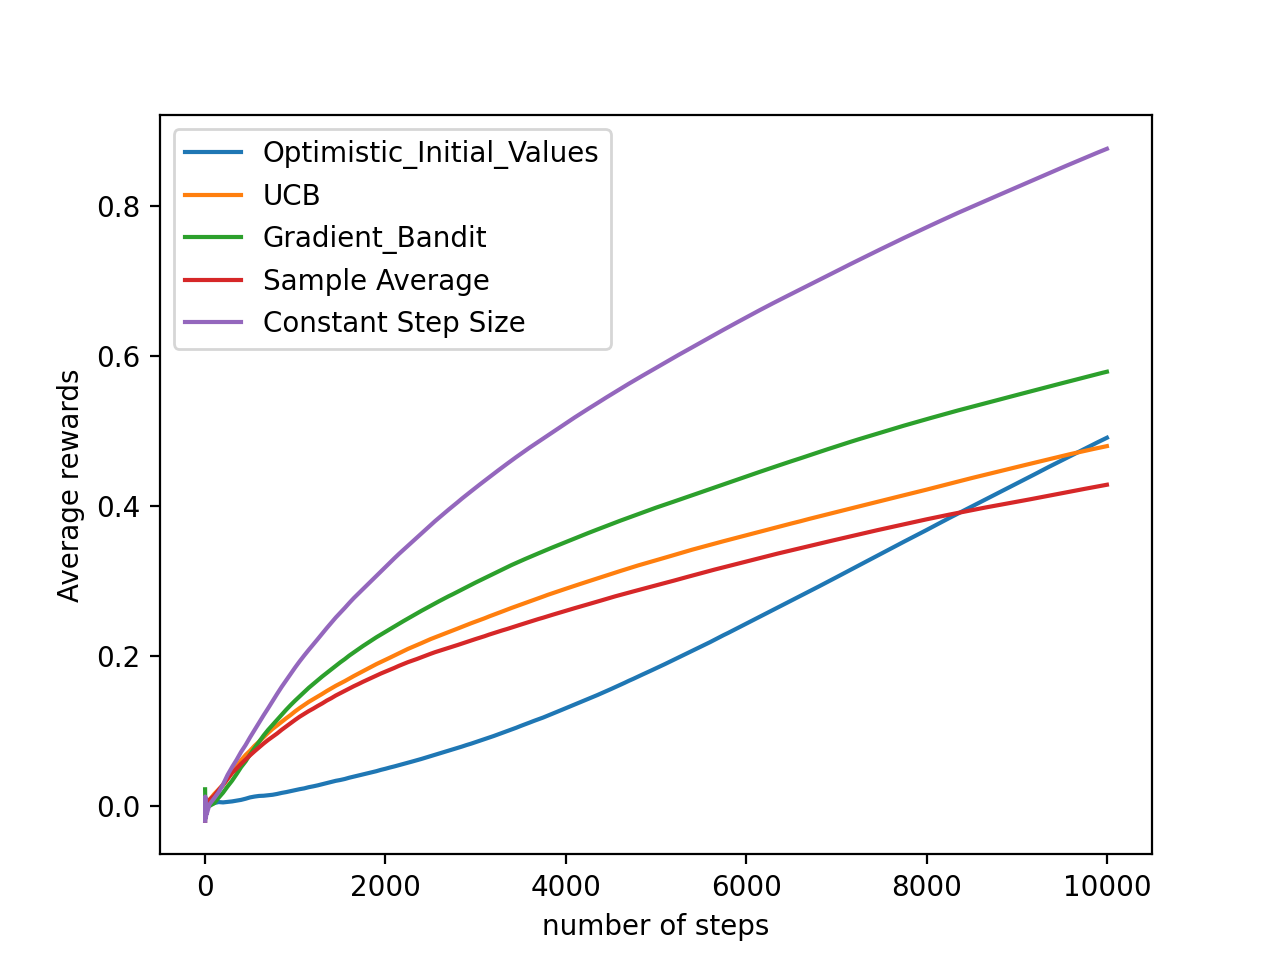
\includegraphics[width=\textwidth]{Figure_7.png}
  \caption{Performance of Sample Average with Optimistic initial methods(blue,$Q_0=$5), UCB(orange,c=1), Gradient bandit method(green,$\alpha$=0.25), Sample average method(red), constant step size(purple,$\alpha$=0.1) in first 10000 steps}
\end{figure}

\pagebreak

\section{Extra Credit Work}
\subsection{Exercise 2.6}
There is a spikes in the early part of the curve for the optimistic method indicates there is higher chance for it to select the optimal action. In optimistic method, each action start with a Q value much larger than the actual q value and each action will result in decrease in Q value of corresponding action. And since optimal has a higher mean, $ Q_{optimal}$ will likely decrease slower than other $Q_{OtherAction}$, resulting in a higher chance to be select again. 

\subsection{Exercise 2.7}
In case of only two actions, let the two action denote by a and b, we have\\
\begin{flalign*}
Pr\{A_t=a\} &= \frac{e^{H_t(a)}}{e^{H_t(a)}+e^{H_t(b)}}  \\
                  &= \frac{1}{1+e^{H_t(b)-H_t(a)}}\\
                  &= \frac{L}{1+e^{-k(a-b)}} \quad \mbox{where L=k=1}
\end{flalign*}
The last line show that it takes the same form as a logistic function


\pagebreak
\begin{thebibliography}{9}

\bibitem{latexcompanion} 
Wikipedia
\textit{Multi-armed bandit}. 


\bibitem{greedy} 
Richard S. Sutton and Andrew G. Barto. 
\textit{Reinforcement Learning: An Introduction}, 2014, 2015, 2016, 2017

\end{thebibliography}

\end{document}

